\documentclass[12pt]{article}

\usepackage[margin=1.5cm]{geometry}
\usepackage{fontspec}
\usepackage{natbib}
\usepackage{graphicx}
\usepackage{amsmath}
\usepackage{unicode-math}
\usepackage[hidelinks]{hyperref}
\usepackage{tikz}
\usetikzlibrary{calc, arrows.meta}

\defaultfontfeatures{Mapping=tex-text,Scale=MatchLowercase}
\setmainfont{Libertinus Serif}
\setsansfont{Libertinus Sans}
\setmonofont{Source Code Pro}
\setmathfont{Libertinus Math}

\newcommand{\iu}{\mathrm{i}}

\title{Hyperbolic Tilings via Group Theory and Automata}
\author{Shengyi Wang}
\begin{document}
\maketitle

\begin{center}
  \includegraphics[width=\textwidth, draft=true]{Hyp552.eps}
\end{center}

\section{Introduction}

The figure on the cover page is a hyperbolic tiling of the Poincar\'e
disk, which is a model of the hyperbolic plane. If the readers are
reading a PDF version of this article, they can zoom in the cover
figure to explore the exquisite detail on the boundary: there are more
than $179,900$ black triangles in total.

In this article I briefly introduce the mathematical principles behind
the figure and explain the algorithm which generates it, just like
\citep{silvio1992}. The generation of these types of triangular tiling
graphics is the combination of geometry, group theory and
deterministic finite automata. Nothing here is new. I just want to
elucidate the elegance of mathematics hidden beneath this stunning
figure.
 
\section{Hyperbolic Geometry}
\begin{figure}[htbp]
  \centering
  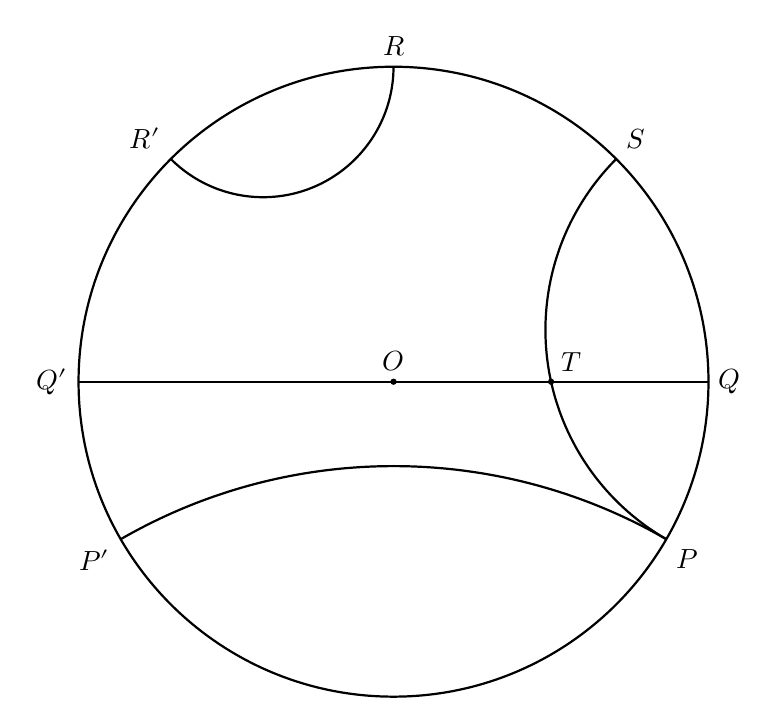
\begin{tikzpicture}[scale=4, thick]
    \draw (0, 0) circle [radius=1];
    \draw (-1, 0) -- (1, 0);
    \draw (-30:1) arc [start angle=60, end angle=120, radius=sqrt(3)];
    \draw (45:1) arc [start angle=135, end angle=240, radius=sqrt(6)+sqrt(3)-sqrt(2)-2];
    \draw (0, 1) arc [start angle=0, end angle=-135, radius=sqrt(2)-1];
    \fill (0, 0) circle [radius=0.01];
    \fill (0.500208, 0) circle [radius=0.01];
    \draw (0.500208, 0) node [anchor=south west] {$T$};
    \draw (0, 0) node [anchor=south] {$O$};
    \draw (0, 1) node [anchor=south] {$R$};
    \draw (135:1) node [anchor=south east] {$R'$};
    \draw (45:1) node [anchor=south west] {$S$};
    \draw (1, 0) node [anchor=west] {$Q$};
    \draw (-1, 0) node [anchor=east] {$Q'$};
    \draw (-30:1) node [anchor=north west] {$P$};
    \draw (210:1) node [anchor=north east] {$P'$};
  \end{tikzpicture}
  \caption{Hyperbolic Straight Lines in the Poincar\'e Disk $\mathbb{D}$}
  \label{fig:hyplines}
\end{figure}

Hyperbolic geometry is a non-Euclidean geometry which satisfies all of
Euclid's postulates except the parallel postulate. The parallel
postulate in hyperbolic geometry is: For any given infinite straight
line $L$ and point $P$ not on $L$, in the plane containing both $L$
and $P$ there are \emph{at least two} distinct infinitely extending
straight lines through $P$ that do not intersect $L$.


The Poincar\'e disk is one of many models of 2-dimensional hyperbolic
geometry (a.k.a.\ \emph{hyperbolic plane}). A \emph{model} means a
choice of an underlying space, together with a choice of the
representation of basic geometric objects, such as points and lines,
in this space. The underlying space of the Poincar\'e disk model is
the open unit disk
\begin{equation}
  \mathbb{D} = \{(x, y) \in \mathbb{R}^2\mid x^2 + y^2 < 1\}
\end{equation}
The points in the Poincar\'e disk are the interior points of the unit
circle. The straight lines are circular arcs which are orthogonal to
the unit circle. For example, the lines $PP'$, $QQ'$, $RR'$ and $PS$
in Figure~\ref{fig:hyplines} are all ``straight'' lines which meet the
rim at right angles. Notice that if a line passes through the center
$O$ like $QQ'$, it remains straight. This is the special case of a
``circular arc'' whose radius is infinite. The points on the rim do
not belong to $\mathbb{D}$. So lines $PP'$ and $PS$ are \emph{limiting
parallel}: They never touch, but their points get closer and closer
together. There are many other pairs of lines, like $PP'$ and $QQ'$,
or $PP'$ and $RR'$, that are totally disjoint or \emph{ultraparallel},
in the sense that their points never become arbitrarily close. This
model does satisfy the parallel postulate in hyperbolic geometry:
through a point $T$ which is not on line $PP'$, lines $PS$ and $QQ'$
both do not intersect $PP'$. Actually through $T$ there are an
infinite number of coplanar lines that do not intersect $PP'$. From
now, we no longer distinguish the Poincar\'e disk model $\mathbb{D}$
and the hyperbolic plane.


Then it is time to consider some quantitative properties of the
hyperbolic plane. Any point in $\mathbb{D}$ can be seen as a complex
number $z=x + \iu y$ satisfying $\lvert z \rvert < 1$. For any two
points $w, z \in \mathbb{D}$, the \emph{hyperbolic distance} between
$w$ and $z$ is defined by:
\begin{equation}\label{eqn:distance}
  d(w, z) = 2\tanh^{-1}\left\lvert\frac{w-z}{1-w\overline{z}}\right\rvert
\end{equation}
where $\tanh^{-1}(x) = \dfrac{1}{2}\ln\dfrac{1+x}{1-x}$, $\lvert
\cdot\rvert$ is the complex absolute value, and $\overline{z}$ is the
complex conjugate. It is easy to see $\displaystyle\lim_{z\rightarrow
  1}d(0,z)=\infty$, which means the hyperbolic distance from the
center to the rim of $\mathbb{D}$ is infinity. Intuitively, if a man
living on $\mathbb{D}$ walks from the center to the rim at a constant
pace, he would never reach the rim. From an outsider's view, he walks
slower and slower while getting smaller and smaller. For this man, the
$\mathbb{D}$ is the whole infinite world! In contrast, the hyperbolic
angles in $\mathbb{D}$ are just Euclidean angles.


\begin{figure}[htbp]
  \centering
  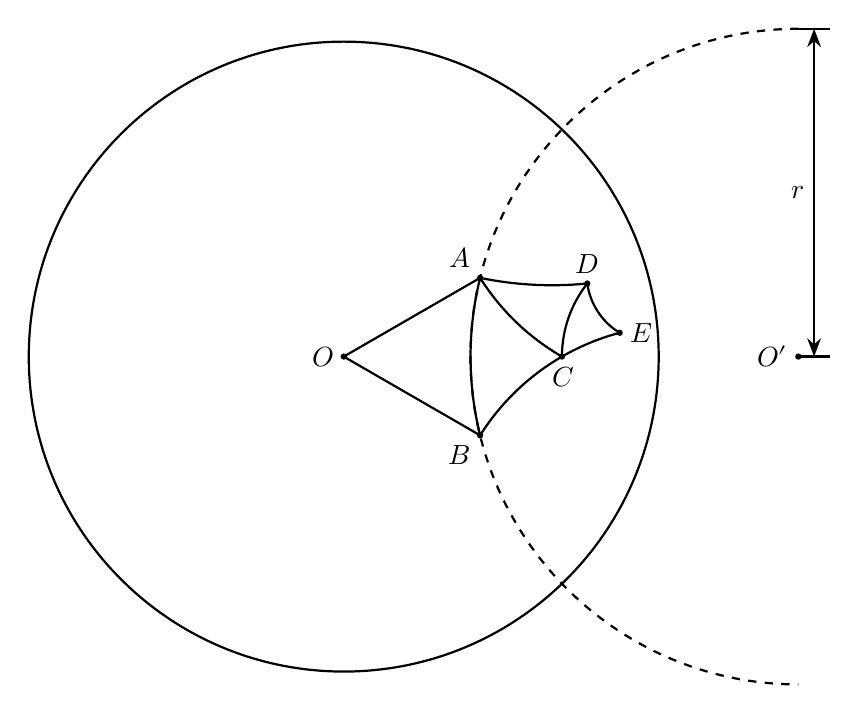
\begin{tikzpicture}[scale=4, thick, >=Stealth]
    \draw (0, 0) circle [radius=1];
    \draw[dashed] (1.44338, 1.04083) arc [start angle=90, end angle=270, radius=1.04083];
    %% \draw[dashed] (1.44338, 0) circle [radius=1.04083];
    \draw (0, 0) -- (0.433013, -0.25) arc [start angle=193.898, end angle=166.102, radius=1.04083] -- cycle;
    \draw (0.433013, 0.25) arc [start angle=-147.796, end angle=-120, radius=0.75055];
    \draw (0.433013, 0.25) arc [start angle=-101.694, end angle=-84.3153, radius=1.12757];
    \draw (0.69282, 0) arc [start angle=180, end angle=141.787, radius=0.375278];
    \draw (0.773237, 0.232143) arc [start angle=-172.111, end angle=-121.28, radius=0.218239];
    \draw (0.433013, -0.25) arc [start angle=147.796, end angle=104.822, radius=0.750555];
    \fill (0, 0) circle [radius=0.01];
    \fill (1.44338, 0) circle [radius=0.01];
    \fill (0.433013, 0.25) circle [radius=0.01];
    \fill (0.433013, -0.25) circle [radius=0.01];
    \fill (0.69282, 0) circle [radius=0.01];
    \fill (0.773237, 0.232143) circle [radius=0.01];
    \fill (0.876095, 0.0755814) circle [radius=0.01];
    \draw (1.44338, 0) node [anchor=east] {$O'$};
    \draw (0, 0) node [anchor=east] {$O$};
    \draw (0.433013, 0.25) node [anchor=south east] {$A$};
    \draw (0.433013, -0.25) node [anchor=north east] {$B$};
    \draw (0.69282, 0) node [anchor=north] {$C$};
    \draw (0.773237, 0.232143) node [anchor=south] {$D$};
    \draw (0.876095, 0.0755814) node [anchor=west] {$E$};
    \draw[<->] (1.49338, 0) -- node[left] {$r$} (1.49338, 1.04083);
    \draw (1.44338, 0) -- (1.54338, 0);
    \draw (1.44338, 1.04083) -- (1.54338, 1.04083);
  \end{tikzpicture}
  \caption{Triangles and Reflections of the Hyperbolic Plane $\mathbb{D}$}
  \label{fig:tri}
\end{figure}


Analogous to reflection in the Euclidean plane, reflection in the
hyperbolic plane is the inversion of a circle. Take
Figure~\ref{fig:tri} as an example, an inversion with respect to a
reference circle with center $O'$ and radius $r$ maps a point $O$ to
point $C$, which lies on the ray from $O'$ through $O$ such that
\begin{equation}\label{eqn:inversion}
  \lVert O'O \rVert \times \lVert O'C \rVert= r^2
\end{equation}
where $\lVert \cdot \rVert$ is the Euclidean distance. The same
inversion also takes $C$ back to $O$ since
equation~\eqref{eqn:inversion} is symmetric. Inversion has many nice
properties. It maps circles or lines to other circles or lines and it
also preserves the angles between crossing curves. More importantly,
it preserves the hyperbolic distance defined in
\eqref{eqn:distance}. For example, we have $d(O, A)=d(A, C)$ in
Figure~\ref{fig:tri}. So the \emph{hyperbolic reflection} with respect
to a hyperbolic line $AB$ is the inversion with respect to the circle
$O'$. Similarly, line $AC$ reflects $B$ to $D$ and line $CD$ reflects
$A$ to $E$. So all triangles in Figure~\ref{fig:tri} are congruent:
their corresponding sides are equal in hyperbolic length, and their
corresponding angles are equal in measure. Actually all triangles on
the cover figure, no matter black or white, are congruent. They are
all generated by sequences of hyperbolic reflections across the sides
of a single, initial triangle. They form a triangular tiling of the
hyperbolic plane $\mathbb{D}$.

\section{M\"obius Triangle and Triangle Group}

The triangle that can be used to tile the entire hyperbolic plane
$\mathbb{D}$ through reflections in its edges without any gaps or
overlaps is called M\"obius triangle. A M\"obius triangle can be
represented by a triple of positive integers $(p, q, r)$ which
satisfies the following condition:
\begin{equation}\label{eqn:mobtri}
  \frac{1}{p} + \frac{1}{q} + \frac{1}{r} < 1
\end{equation}
The triple $(p, q, r)$ means the vertex angles of a M\"obius triangle
are $\pi/p$, $\pi/q$, and $\pi/r$ repectively. The
equation~\eqref{eqn:mobtri} just reveals the fact that the sum of the
angles of any hyperbolic triangle is strictly less than a straight
angle. The M\"obius triangle of the cover figure is $(5, 5, 2)$. The
triple can be determined by the number of surrounding triangles of
each vertex, which is 10, 10, and 4 respectively in this case.

The cover figure can be seen as the geometric realization of a certain
kind of hyperbolic reflection group: triangle group.

\bibliographystyle{abbrv}
\bibliography{triangle}

\end{document}
